\subsubsection{Servidor}

\begin{description}

\item[Gestão e manipulação de dados:]
Os servidores têm responsabilidade de se registar no \textit{master} assim que estejam activos. Têm como função guardar e alterar os objectos partilhados, deste modo podem ser vistos como um repositório. De um modo mais especifico, cada servidor, além dos objectos nativos com número de acessos considerado normal, faz ainda a distinção entre objecto especiais, objectos para replicar, objectos para migrar e objectos especiais provenientes de outros servidores. Quanto aos objectos para replicar, mantêm-se numa fila própria para o efeito até a replicação ser efectivamente concluída. Este processo de replicação só não é instantâneo quando o servidor responsável por receber a réplica \footnote{$ \textit{hash(uid+1) mod n} $} está indisponível, sendo o processo concluído quando o servidor estiver novamente disponível. Em relação aos dados para migrar, o mecanismo de fila de espera é igual, mas o servidor de destino é escolhido aleatoriamente pelo \textit{master}, entre os que estão disponíveis. Quando um objecto é alterado com sucesso, é da responsabilidade do servidor encaminhar essa informação até à sua réplica e também ao coordenador dessa transacção.O tipo PadInt é composto por um inteiro que corresponde ao seu valor, pelos contadores de acessos (\textit{read}/\textit{write}), pelos \textit{timestamps} das últimas versões que fizeram escritas/leituras e \textit{commits} com sucesso, e por um $\textit{enum\{TEMPORARY, DELETE, MIGRATE, NONE\}}$. Cada objecto é guardado numa tabela de dispersão criada especificamente para gerir intervalos de uids. Cada uid serve de \textit{key} para aceder ao objecto na tabela. 

\item[Marcação de dados a migrar:]
Cada vez que é feita uma escrita ou leitura a um PadInt é chamada uma função que incrementa  o número de acessos a esse objecto em específico. A métrica escolhida para contabilizar o número de acessos consiste em incrementar duas unidades no caso de se efectuar uma leitura e três no caso ser uma escrita. Quando a média do número de acessos por segundo (1000 acessos em 3 segundos) é excedida, o objecto é considerado especial pelo servidor. Note-se que a verificação do número de acessos por segundo só é feita em cada \textit{read}/\textit{write}, ou seja, o sistema só verifica quando realmente está a usar aquele objecto, minimizando assim o trabalho computacional. Um determinado objecto especial só é escolhido para migrar caso o número de objectos especiais existentes nesse servidor for maior que um. Quando isto acontece, o servidor notifica o \textit{master} para que este último lhe indique o endereço de um outro servidor disponível para receber o PadInt em questão. Este ultimo mecanismo nunca migra um objecto extremamente acedido para a mesma localização da sua réplica, senão iria perder-se o conceito de redundância. Isto é vantajoso na medida em que os objectos extremamente acedidos ficam distribuídos pelos diferentes servidores, permitindo assim o balanceamento de carga do sistema. Note-se ainda que o número de acessos por segundo pode ser adaptado aos mais diversos tipos de sistemas, de modo a maximizar o desempenho.

\begin{figure}[htb]
\centering
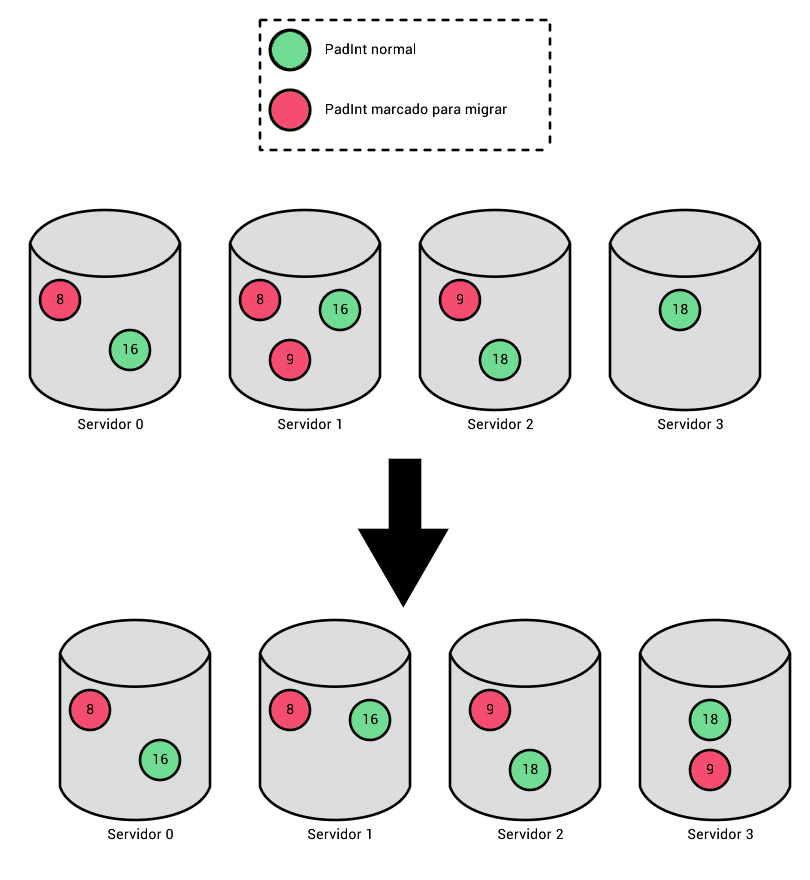
\includegraphics[width=0.5\textwidth]{migracao.png}
\caption{\label{fig:migracao}Balanceamento de carga.}
\end{figure}

\item[Versões tentativas:]
Cada coordenador gere ainda um conjunto de tentativas transaccionais (versões tentativas dos dados antes do \textit{commit}), para quando tentar fazer \textit{commit} ter essa informação disponível. Esta informação é útil porque o coordenador verifica se uma determinada transacção depende de outra para o \textit{commit} ter sucesso, e se depender, fica à espera da respectiva transacção. Assim permite-se que as transacções esperem, ao invés de abortarem devido às dependências com outras transacções. A grande vantagem desta abordagem é o paralelismo que a mesma permite, uma vez que podem executar-se bastantes transacções em cadeia, no qual o conhecimento das dependências permite que todas fazem \textit{commit} com sucesso. O facto do contexto estar nos servidores também é uma vantagem, porque permite que, se um servidor falhar, o cliente continue a executar a transacção, no servidor replicado de forma invisível, ou seja, o cliente não nota diferença no desempenho do sistema. 

\end{description}